\documentclass[border=8pt]{standalone}
\usepackage[utf8]{inputenc}
\usepackage{amsmath}
\usepackage{tikz}
\usetikzlibrary{arrows.meta,positioning,fit,backgrounds,shapes.geometric,calc,decorations.pathreplacing}

% ── colour palette ─────────────────────────────────────────────
\definecolor{cInput}{HTML}{F0F4F8}
\definecolor{cMod1}{HTML}{D1FAE5}
\definecolor{cMod2}{HTML}{DBEAFE}
\definecolor{cMod3}{HTML}{FEF3C7}
\definecolor{cMod4}{HTML}{FCE7F3}
\definecolor{cBlue}{HTML}{2563EB}
\definecolor{cGreen}{HTML}{059669}
\definecolor{cAmber}{HTML}{D97706}
\definecolor{cPink}{HTML}{DB2777}
\definecolor{cGray}{HTML}{4B5563}
\definecolor{cDark}{HTML}{1F2937}

\tikzset{
  modbox/.style={
    draw, rounded corners=6pt, thick,
    minimum width=5.5cm, minimum height=1.2cm,
    text centered, font=\sffamily\bfseries\large,
  },
  subbox/.style={
    draw, rounded corners=4pt, thick,
    minimum width=4cm, minimum height=0.9cm,
    text centered, font=\sffamily,
  },
  tinybox/.style={
    draw, rounded corners=4pt, thick,
    minimum width=3.2cm, minimum height=0.8cm,
    text centered, font=\sffamily\small,
  },
  io/.style={
    draw, rounded corners=4pt, thick, dashed,
    minimum width=3.5cm, minimum height=0.9cm,
    text centered, font=\sffamily\small,
  },
  arr/.style={
    -{Stealth[length=3mm]}, thick, draw=cGray,
  },
  dashedarr/.style={
    -{Stealth[length=3mm]}, thick, dashed, draw=cGray,
  },
  modlabel/.style={
    font=\sffamily\footnotesize, text=cGray, fill=white, inner sep=1pt,
  },
}

\begin{document}
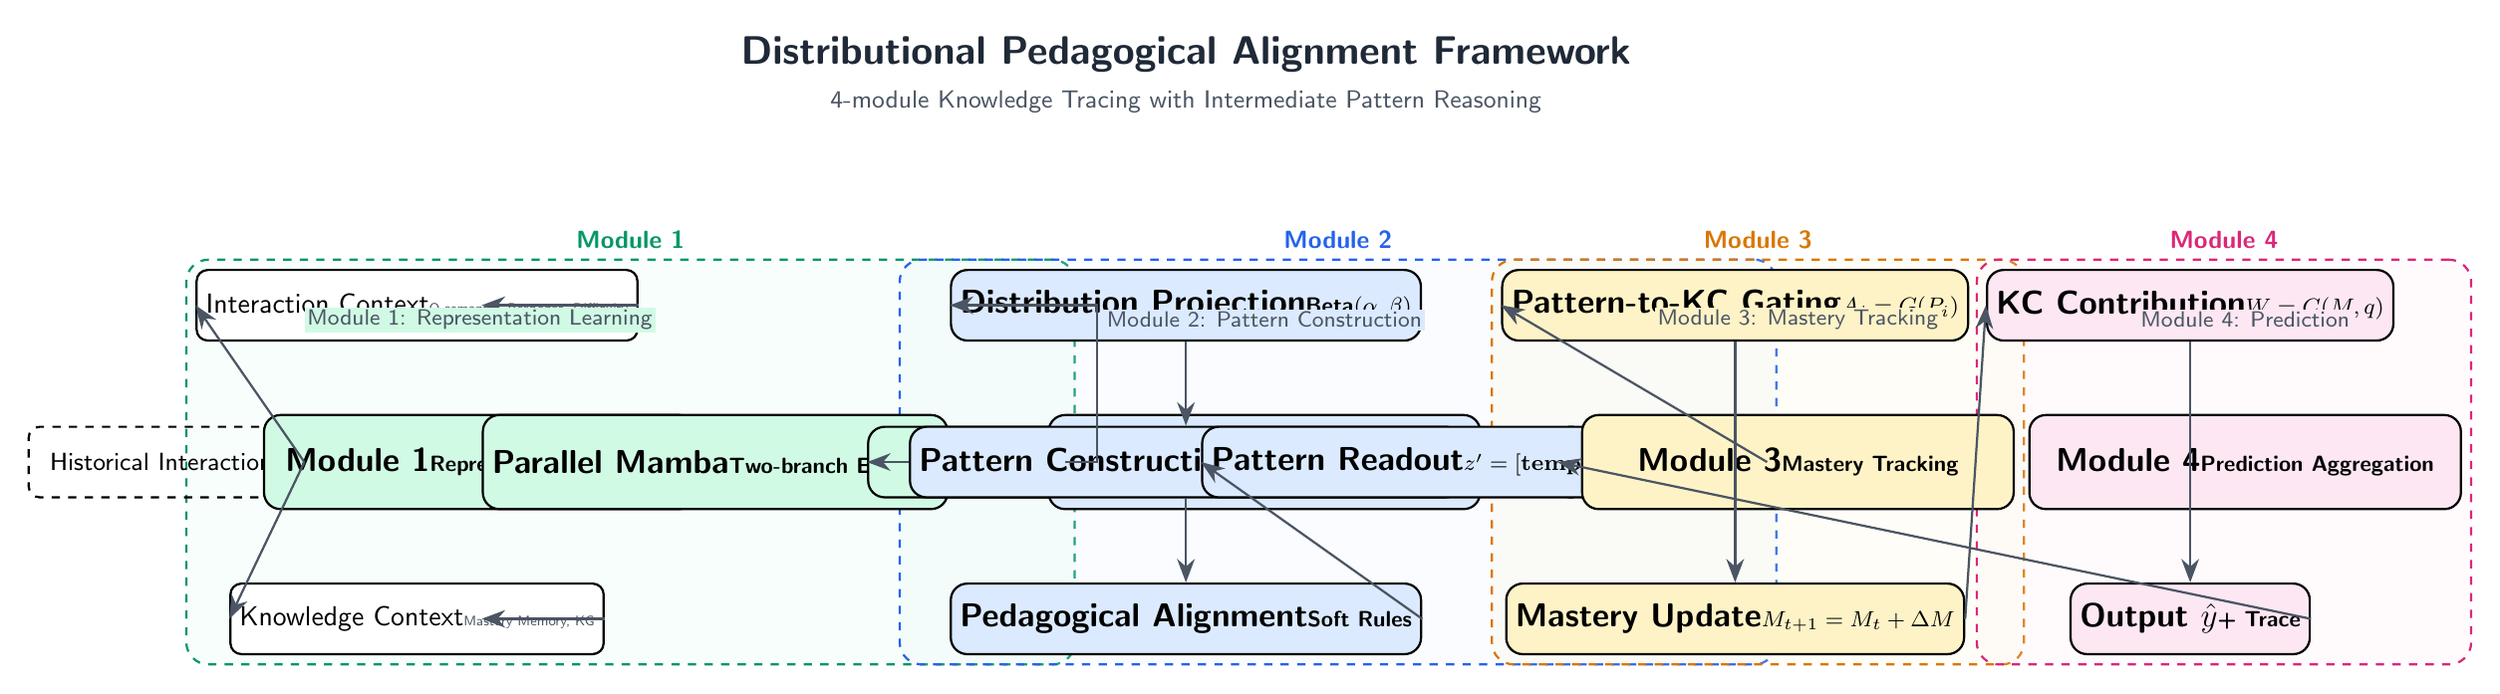
\begin{tikzpicture}[>=Stealth]

% ═══════════════════════════════════════════════════════════════
%  ROW COORDINATES  (y):  input row = 0
% ═══════════════════════════════════════════════════════════════

% ── I/O ──────────────────────────────────────────────────────
\node[io] (input) at (-1,0)
  {Historical\\[-2pt] Interactions};
\node[io] (output) at (18.5,0)
  {Prediction\\[-2pt] $\hat{y}$ + Trace};

% ═══════════════════════════════════════════════════════════════
%  MODULE 1 – Interaction Representation Learning
% ═══════════════════════════════════════════════════════════════
\node[modbox, fill=cMod1] (m1) at (3,0)
  {Module 1\\\footnotesize Representation Learning};

\node[subbox, fill=white] (ictx) at (2.2, 2.0)
  {Interaction Context\\[-2pt]{\tiny\color{cGray} Q-semantic, Response, Difficulty}};
\node[subbox, fill=white] (kctx) at (2.2,-2.0)
  {Knowledge Context\\[-2pt]{\tiny\color{cGray} Mastery Memory, KG}};

\node[modbox, fill=cMod1, minimum width=4.2cm] (mamba) at (6,0)
  {Parallel Mamba\\[-2pt]{\footnotesize Two-branch Encoder}};

\node[modbox, fill=cMod1, minimum width=2.5cm, minimum height=0.9cm] (fusion) at (9.2,0)
  {Fusion\\[-2pt]{\footnotesize $z_t$}};

% ── arrows inside M1 ──
\draw[arr] (input.east) -- (ictx.west);
\draw[arr] (input.east) -- (kctx.west);
\draw[arr] (ictx.east) -- (mamba.west |- ictx);
\draw[arr] (kctx.east) -- (mamba.west |- kctx);
\draw[arr] (mamba.east) -- (fusion.west);

% ═══════════════════════════════════════════════════════════════
%  MODULE 2 – Distributional Pedagogical Alignment
% ═══════════════════════════════════════════════════════════════
\node[modbox, fill=cMod2] (m2) at (13,0)
  {Module 2\\\footnotesize Pattern Construction};

\node[modbox, fill=cMod2, minimum width=4.2cm, minimum height=0.9cm] (proj) at (12, 2.0)
  {Distribution Projection\\[-2pt]{\footnotesize Beta$(\alpha,\beta)$}};
\node[modbox, fill=cMod2, minimum width=4.2cm, minimum height=0.9cm] (pattern) at (12, 0)
  {Pattern Construction\\[-2pt]{\footnotesize Multi-view Operators}};
\node[modbox, fill=cMod2, minimum width=4.2cm, minimum height=0.9cm] (align) at (12,-2.0)
  {Pedagogical Alignment\\[-2pt]{\footnotesize Soft Rules}};

\node[modbox, fill=cMod2, minimum width=3cm, minimum height=0.9cm] (readout) at (15.8,0)
  {Pattern Readout\\[-2pt]{\footnotesize $z' = [\textrm{temp},\textrm{same},\textrm{pre},\textrm{nbr}]$}};

% ── arrows inside M2 ──
\draw[arr] (fusion.east) -- ++(0.4,0) |- (proj.west);
\draw[arr] (proj.south) -- (pattern.north);
\draw[arr] (pattern.south) -- (align.north);
\draw[arr] (align.east) -- (readout.west);

% ═══════════════════════════════════════════════════════════════
%  MODULE 3 – Mastery State Tracking
% ═══════════════════════════════════════════════════════════════
\node[modbox, fill=cMod3] (m3) at (19.8,0)
  {Module 3\\\footnotesize Mastery Tracking};

\node[modbox, fill=cMod3, minimum width=4.2cm, minimum height=0.9cm] (gating) at (19, 2.0)
  {Pattern-to-KC Gating\\[-2pt]{\footnotesize $A_i = G(P_i)$}};
\node[modbox, fill=cMod3, minimum width=4.2cm, minimum height=0.9cm] (update) at (19,-2.0)
  {Mastery Update\\[-2pt]{\footnotesize $M_{t+1} = M_t + \Delta M$}};

% ── arrows inside M3 ──
\draw[arr] (readout.east) -- (gating.west);
\draw[arr] (gating.south) -- (update.north);

% ═══════════════════════════════════════════════════════════════
%  MODULE 4 – Prediction Aggregation
% ═══════════════════════════════════════════════════════════════
\node[modbox, fill=cMod4] (m4) at (25.5,0)
  {Module 4\\\footnotesize Prediction Aggregation};

\node[modbox, fill=cMod4, minimum width=4.2cm, minimum height=0.9cm] (kcContrib) at (24.8, 2.0)
  {KC Contribution\\[-2pt]{\footnotesize $W = C(M, q)$}};
\node[modbox, fill=cMod4, minimum width=3cm, minimum height=0.9cm] (pred) at (24.8,-2.0)
  {Output $\hat{y}$\\[-2pt]{\footnotesize + Trace}};

% ── arrows inside M4 ──
\draw[arr] (update.east) -- (kcContrib.west);
\draw[arr] (kcContrib.south) -- (pred.north);
\draw[arr] (pred.east) -- (output.west);

% ═══════════════════════════════════════════════════════════════
%  BOUNDARIES  (regions)
% ═══════════════════════════════════════════════════════════════
\begin{scope}[on background layer]
  \node[draw=cGreen, dashed, thick, rounded corners=8pt,
        fill=cMod1, fill opacity=0.15,
        fit=(m1)(ictx)(kctx)(mamba)(fusion),
        label={[font=\sffamily\small\bfseries, cGreen]above:Module 1}] {};
  \node[draw=cBlue, dashed, thick, rounded corners=8pt,
        fill=cMod2, fill opacity=0.15,
        fit=(m2)(proj)(pattern)(align)(readout),
        label={[font=\sffamily\small\bfseries, cBlue]above:Module 2}] {};
  \node[draw=cAmber, dashed, thick, rounded corners=8pt,
        fill=cMod3, fill opacity=0.15,
        fit=(m3)(gating)(update),
        label={[font=\sffamily\small\bfseries, cAmber]above:Module 3}] {};
  \node[draw=cPink, dashed, thick, rounded corners=8pt,
        fill=cMod4, fill opacity=0.15,
        fit=(m4)(kcContrib)(pred),
        label={[font=\sffamily\small\bfseries, cPink]above:Module 4}] {};
\end{scope}

% ═══════════════════════════════════════════════════════════════
%  INTER-MODULE LABELS
% ═══════════════════════════════════════════════════════════════
\node[modlabel, fill=cMod1] at ($(m1.north)+(0,1.2)$)
  {Module 1: Representation Learning};
\node[modlabel, fill=cMod2] at ($(m2.north)+(0,1.2)$)
  {Module 2: Pattern Construction};
\node[modlabel, fill=cMod3] at ($(m3.north)+(0,1.2)$)
  {Module 3: Mastery Tracking};
\node[modlabel, fill=cMod4] at ($(m4.north)+(0,1.2)$)
  {Module 4: Prediction};

% ═══════════════════════════════════════════════════════════════
%  TITLE
% ═══════════════════════════════════════════════════════════════
\node[font=\sffamily\Large\bfseries, cDark] at (12,5.2)
  {Distributional Pedagogical Alignment Framework};
\node[font=\sffamily\small, cGray] at (12,4.6)
  {4-module Knowledge Tracing with Intermediate Pattern Reasoning};

\end{tikzpicture}
\end{document}
